\documentclass[12pt]{report}

\usepackage[brazil,american]{babel}
\usepackage[utf8]{inputenc}
\usepackage[a4paper, total={6.5in, 9.5in}]{geometry}

\usepackage{titlesec}
\titleformat{\chapter}[display]
  {\normalfont\bfseries}{}{0pt}{\Huge}

\usepackage{url}
\usepackage{graphicx}
\usepackage{authblk}
\usepackage{hyperref}
\usepackage{lipsum}
\usepackage{xcolor}
\usepackage{float}

% \pagecolor[rgb]{0.1,0.1,0.1}
% \color[rgb]{0.9,0.9,0.9}

\begin{titlepage}
    \title{
        
\includegraphics[width=4cm]{img/logo.jpg} \\ 
        \large
        Dep. Ciência da Computação -- Universidade de Brasília (UnB)\\
        CIC0207 - Projeto Interdisciplinar de Licenciatura em Computação \\
        \vfill 
        \vfill
        \LARGE
        \textbf{Portal de Equações Matemáticas de Primeiro e Segundo Grau}
    }

    \author{
        Letícia Dias Soares Alves, 18/0022059\\
        Pedro Henrique de Brito Agnes, 18/0026305
    }
    
    \affil{
        \vfill
        \vfill
        \vfill
        Professora \\
        Dr.a Letícia Lopes Leite
    }

    \date{Brasília\\Dezembro de 2020}

\end{titlepage}

\begin{document}
\maketitle

\selectlanguage{american}
\begin{abstract}
  With the great difficulty that can be observed on math students on school, it's necessary that they have access to some tools meant to help on the understanding of the subject and even awake their interest on it. To solve the problem, the portal of first and second degree equations was developed with the goal to help the students on learning the so feared subject that is used on many others, taking advantage of the interdisciplinarity with physics and chemistry among others.

  The portal have an explanation of the subject, with videos, curiosities, among others. There is also a selection of exercises to help the students to practice what was learned, and also the resolution of each exercise so they can check their answers to see if its right or where they commit a mistake. At last, there is also a page that allows the student to type any equation to see the answer aswell as the graphic to the function that represents it, which can help on the understanding of the equations by itself when used along with the resources of the website.
\end{abstract}

\selectlanguage{brazil}
\begin{abstract}
  Com a grande dificuldade que pode ser observada nos estudantes em matérias de matemática, torna-se necessária a disponibilidade de ferramentas para o auxílio do ensino de forma melhorar o entendimento da matéria e até a despertar o interesse dos alunos. Para solucionar o problema, o portal de equações de primeiro e segundo grau foi desenvolvido com o objetivo de auxiliar os alunos no aprendizado desta matéria tão temida que é utilizada em diversas outras, tomando vantagem da interdisciplinaridade com a física, química e outros.

  O portal contém explicações do conteúdo de equações, com vídeos explicativos, curiosidades, entre outros. Também possui uma seleção de exercícios para ajudar os estudantes a praticar o conhecimento adquirido com a resolução disponível caso o usuário deseje conferir a resposta para ver se acertou ou onde cometeram um erro. Por fim, uma página que permite ao estudante digitar uma equação quealquer para obter a resposta para a mesma, assim como o gráfico da função que a representa, o que pode auxiliar no entendimento das equações em si, quando usado em conjunto com os materiais disponíveis no portal.
\end{abstract}

\tableofcontents
\newpage

\chapter{Introdução}
Na matemática entendemos equações como expressões algébricas que possuem incógnitas representadas por letras (notações mais usadas são: x,y,z,w), e foram criadas há muito tempo atrás para a solução de problemas quando o número é desconhecido. As equações de primeiro (onde o expoente da incógnita é igual a 1) e segundo grau  (onde o expoente da incógnita é igual a 2), desenvolvem um papel muito importante na rotina de alunos e professores, mas que muitas das vezes essas matérias acabam sendo passadas de forma tradicional e mecânica, que pode acabar interferindo na assimilação do conteúdo.

As equações são muito utilizadas no ensino fundamental (onde são ensinadas), caso o aluno não consiga assimilar a matéria, terá muitas dificuldades, pois, este mesmo conteúdo é usado no nível médio e superior. Esse trabalho é desenvolvido com a finalidade de mostrar uma forma alternativa de passar esses conteúdos utilizando ferramentas que mostrem outras formas de apresentar a mesma matéria. Nossa ideia foi desenvolver um software onde o aluno possa escrever a equação desejada e ver a resolução da questão mostrando o passo a passo. 

\chapter{Problema}
É comum atualmente muitos professores usarem metodologias tradicionais (onde o professor é o centro do processo de ensino aprendizagem), e isso acaba afetando todos os alunos que não conseguem se encaixar neste sistema. A tecnologia poderia auxiliar tanto os professores quanto os alunos, pois com o auxílio da tecnologia poderiam ser criadas muitas ferramentas para cada tipo de pessoa, alguns ferramentas com mais textos, imagens, vídeo aulas específicas, ou até mesmo jogos, questionários, etc.

A dificuldade na resolução de equações ao longo do período escolar é natural e se torna presente em muitos alunos, que acabam por perder todo o interesse pela matéria, em especial quando não conseguem encontrar uma aplicabilidade para elas. A baixa capacidade de resolução de equações pode afetar negativamente o desempenho em matérias como física, química e a própria matemática, em que este conteúdo é usado o tempo todo e qualquer pequeno erro já faz com que o aluno perca toda uma questão. O projeto tem como finalidade, a descomplicação do conteúdo por meio de um \textit{website} onde o aluno possa encontrar os recursos necessários para o aprendizado efetivo da matéria.

\chapter{Levantamento de Requisitos}
Durante esta etapa, foi definido que seriam usadas as ferramentas HTML, CSS e Javascript para o desenvolvimento do portal, assim como foi definido que ele seria composto apenas de \textit{front-end} versionado no \href{https://github.com/Pedenite/PILC-eq}{github}, também sendo feito o \textit{deploy} por meio do \href{https://pedenite.github.io/PILC-eq/}{github-pages}. Foi analisado que o portal deveria ter como conteúdo, explicações da matéria considerando o público-alvo, que são jovens de 14 a 18 anos, exemplos de exercícios que variam desde os mais simples aos mais complexos e aplicações para proporcionar um entendimento melhor da matéria ao incluir gráficos e interdisciplinarizar com a física por exemplo e até coisas do mundo real.

\section{Trabalhos Relacionados}
Existem softwares na internet com uma proposta bem similar, como exemplo temos o \href{https://pt.symbolab.com/}{Symbolab} que permite que o usuário digite equações para que seja mostrada a solução detalhada passo a passo para o problema. Porém a ferramenta possui limitação no plano gratuito e não mostra todos os passos para a resolução, mas ela atende problemas mais avançados também como matérias estudadas no ensino superior.

Outro exemplo de um trabalho é o photomath. Trata-se de um aplicativo para smartphones que permite ao usuário apontar a câmera do celular em uma equação matemática e ele assume a responsabilidade de resolver mostrando gráfico, passos para resolução, entre outros. O aplicativo, além de resolver os problemas básicos de equações, também resolve funções mais complexas assim como o site citado acima.

A aplicação de interdisciplinaridade nos conteúdos de matemática já é usada há tempos em universidades em matérias como cálculo de forma a facilitar o entendimento e, principalmente fazer os alunos entenderem o "para quê" do conteúdo e não somente como resolver o problema, o que pode proporcionar um maior interesse pela matéria e fazer com que o conteúdo seja melhor fixado pelos alunos. Nosso objetivo é parecido neste sentido com a adição de ser um portal facilmente acessível pela internet para que qualquer um possa aprender.

\chapter{Esboços das telas}
O software desenvolvido é, de certa forma inspirado no \href{https://pt.symbolab.com/}{Symbolab} e no Photomath, como mencionado anteriormente, que são "calculadoras" avançadas que mostram a resolução passo a passo dos exercícios desde os mais simples até os mais avançados com até matérias do ensino superior. Ao esboçar as telas da aplicação, foi definido que o portal seria composto de pelo menos uma \textit{home}, uma página com a explicação do conteúdo e outra com o modo de calculadora para a resolução de exercícios.

\section{Página inicial}
A página principal do portal foi esboçada de forma bem simples, mostrando apenas uma introdução, detalhes sobre o projeto e um guia básico de utilização da aplicação, assim como links para as outras páginas. Também incluiria referências e informações dos autores como as de contato para que os estudantes possam conferir as fontes, assim como informar sobre erros na aplicação por e-mail, caso encontrem.

\begin{figure}[H]
    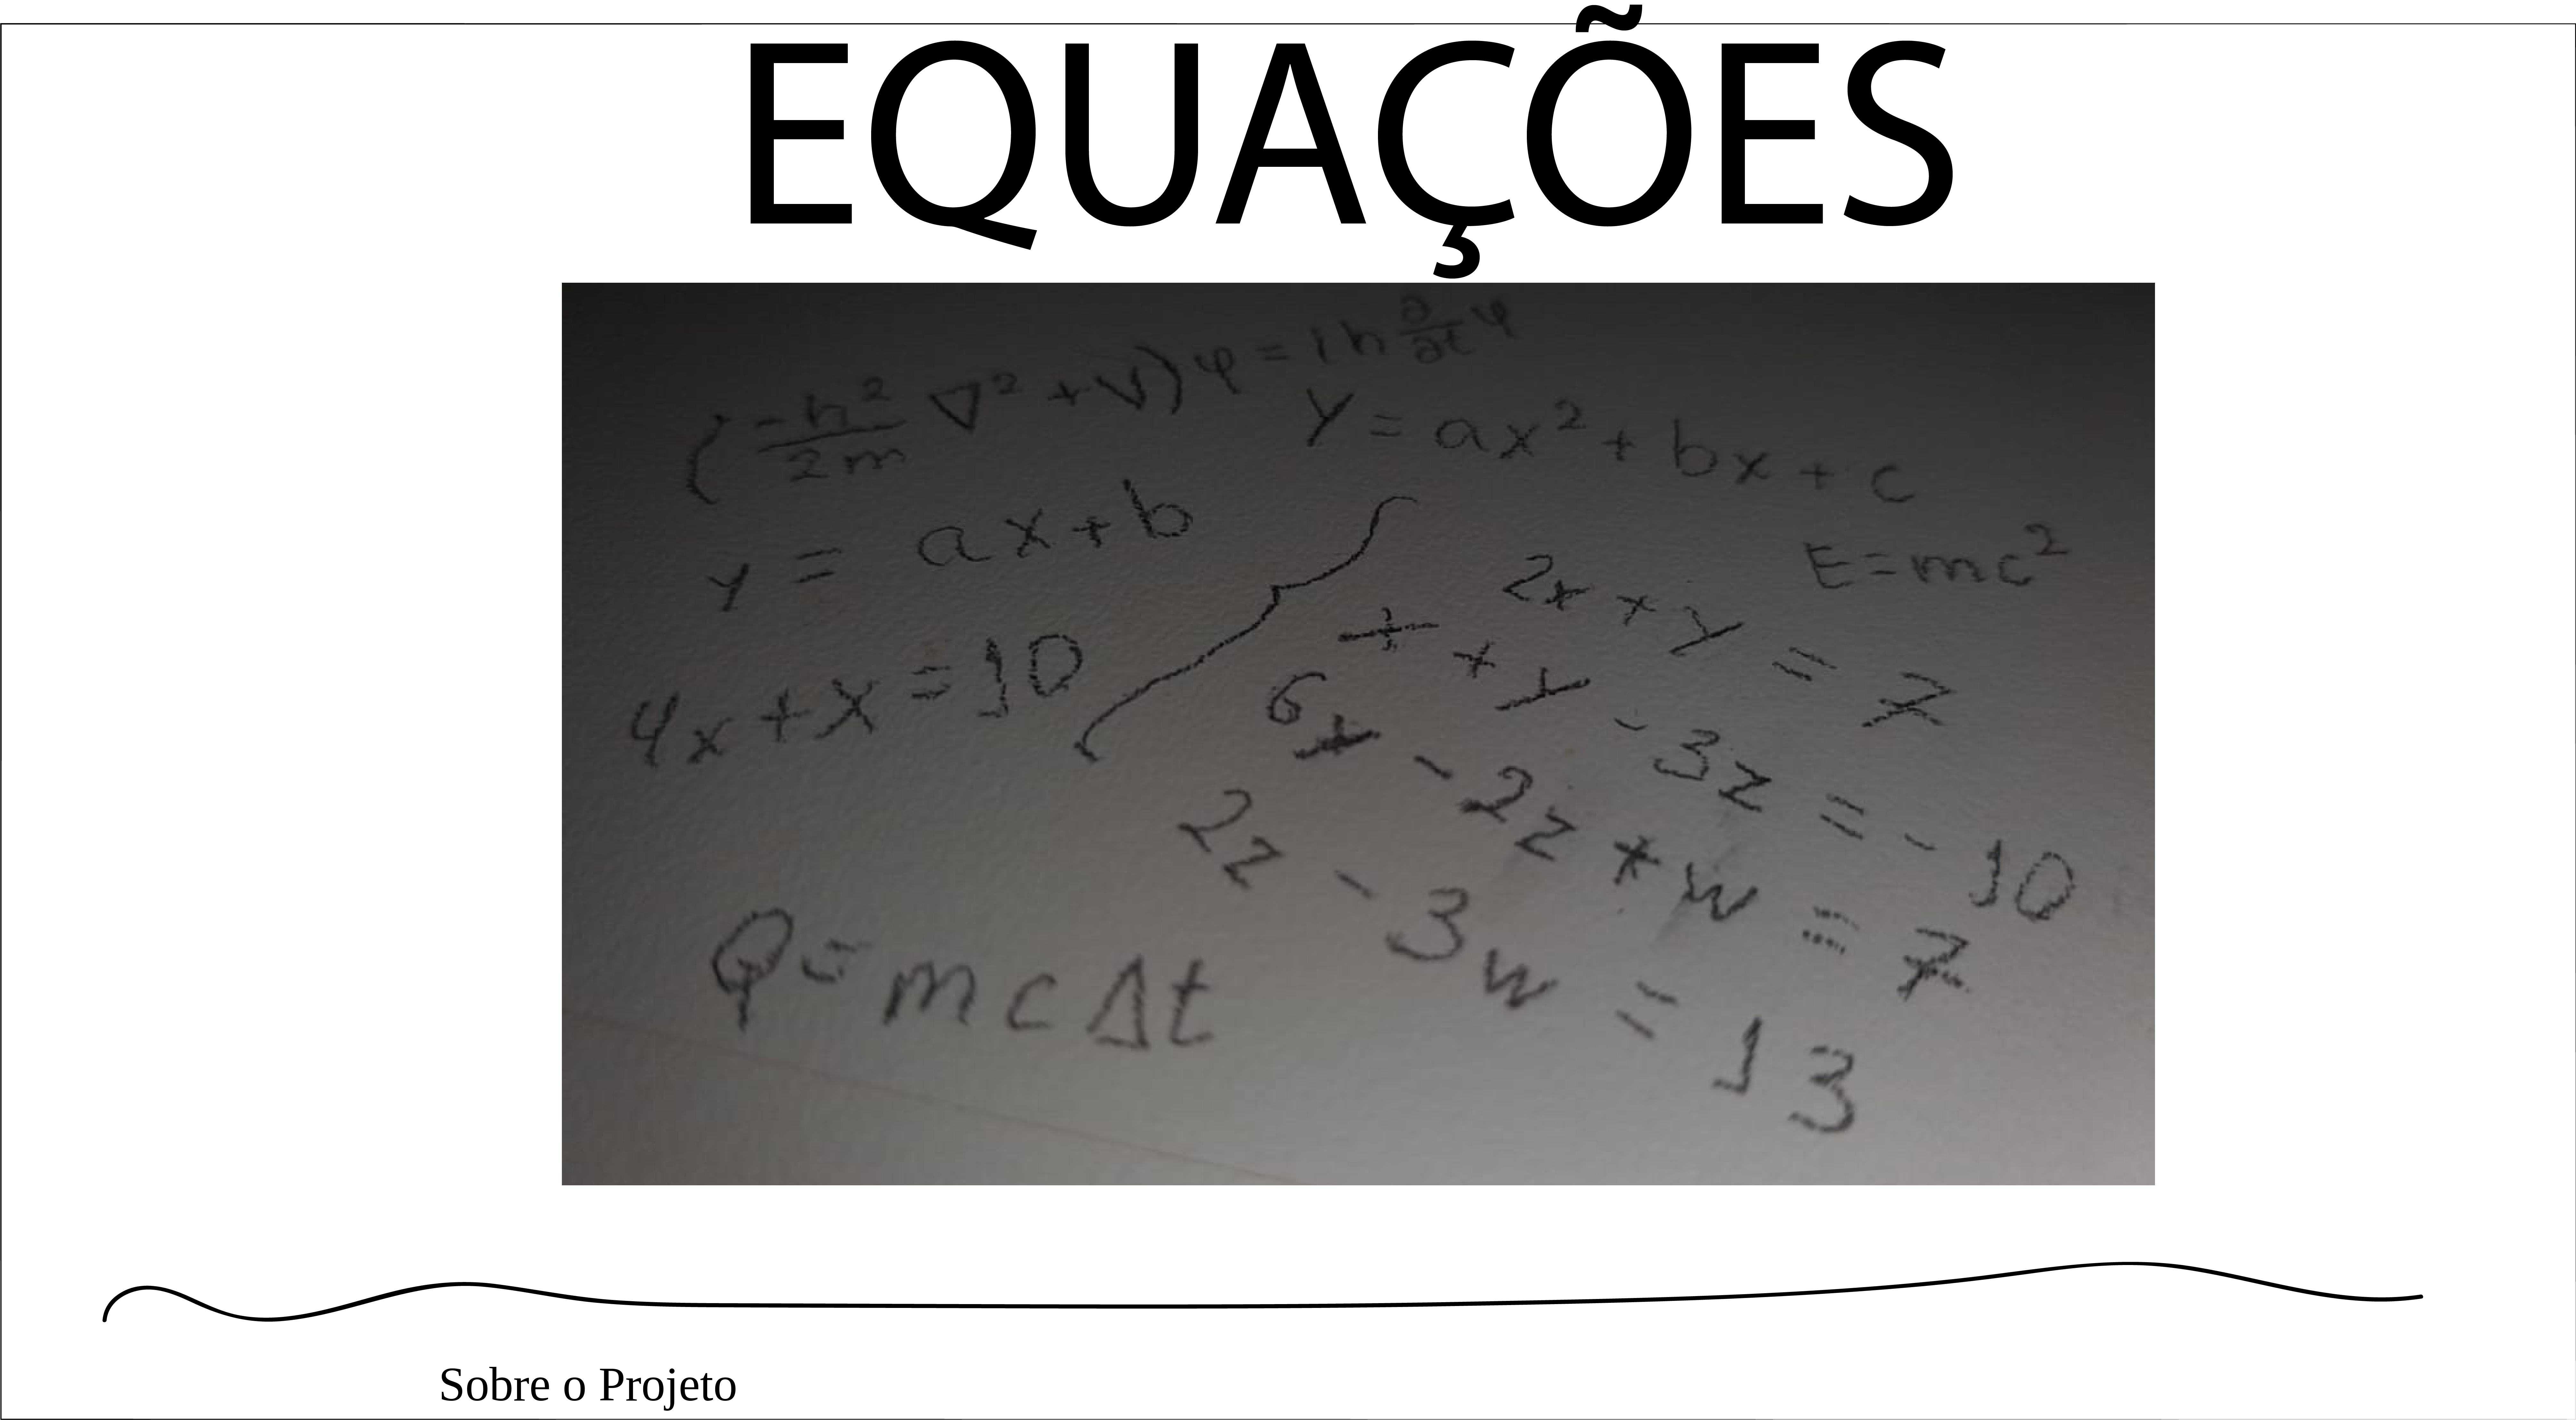
\includegraphics[width=1\textwidth]{img/c.png}
    \caption{Esboço da tela \textit{Home}}
\end{figure}

\section{Exercícios}
A princípio, foi esboçada a segunda tela como de exercícios e explicação do conteúdo, possuindo vídeos, gráficos, exemplos de problemas resolvidos com a opção de clicar em cima para mostrar o passo a passo da resolução da equação se o usuário quiser tentar resolver antes por si só, entre outros. Já havia sido planejado para possuir um "dark mode" para agradar a todo tipo de público que podem ativar/desativar pelo botão na barra de navegação, que apesar de não estar no esboço, está presente na versão final e apenas atera a aparência do portal sem mudar as posições de nenhum elemento, alterando mesmo apenas o esquema de cores para mais escuros.

\begin{figure}[H]
    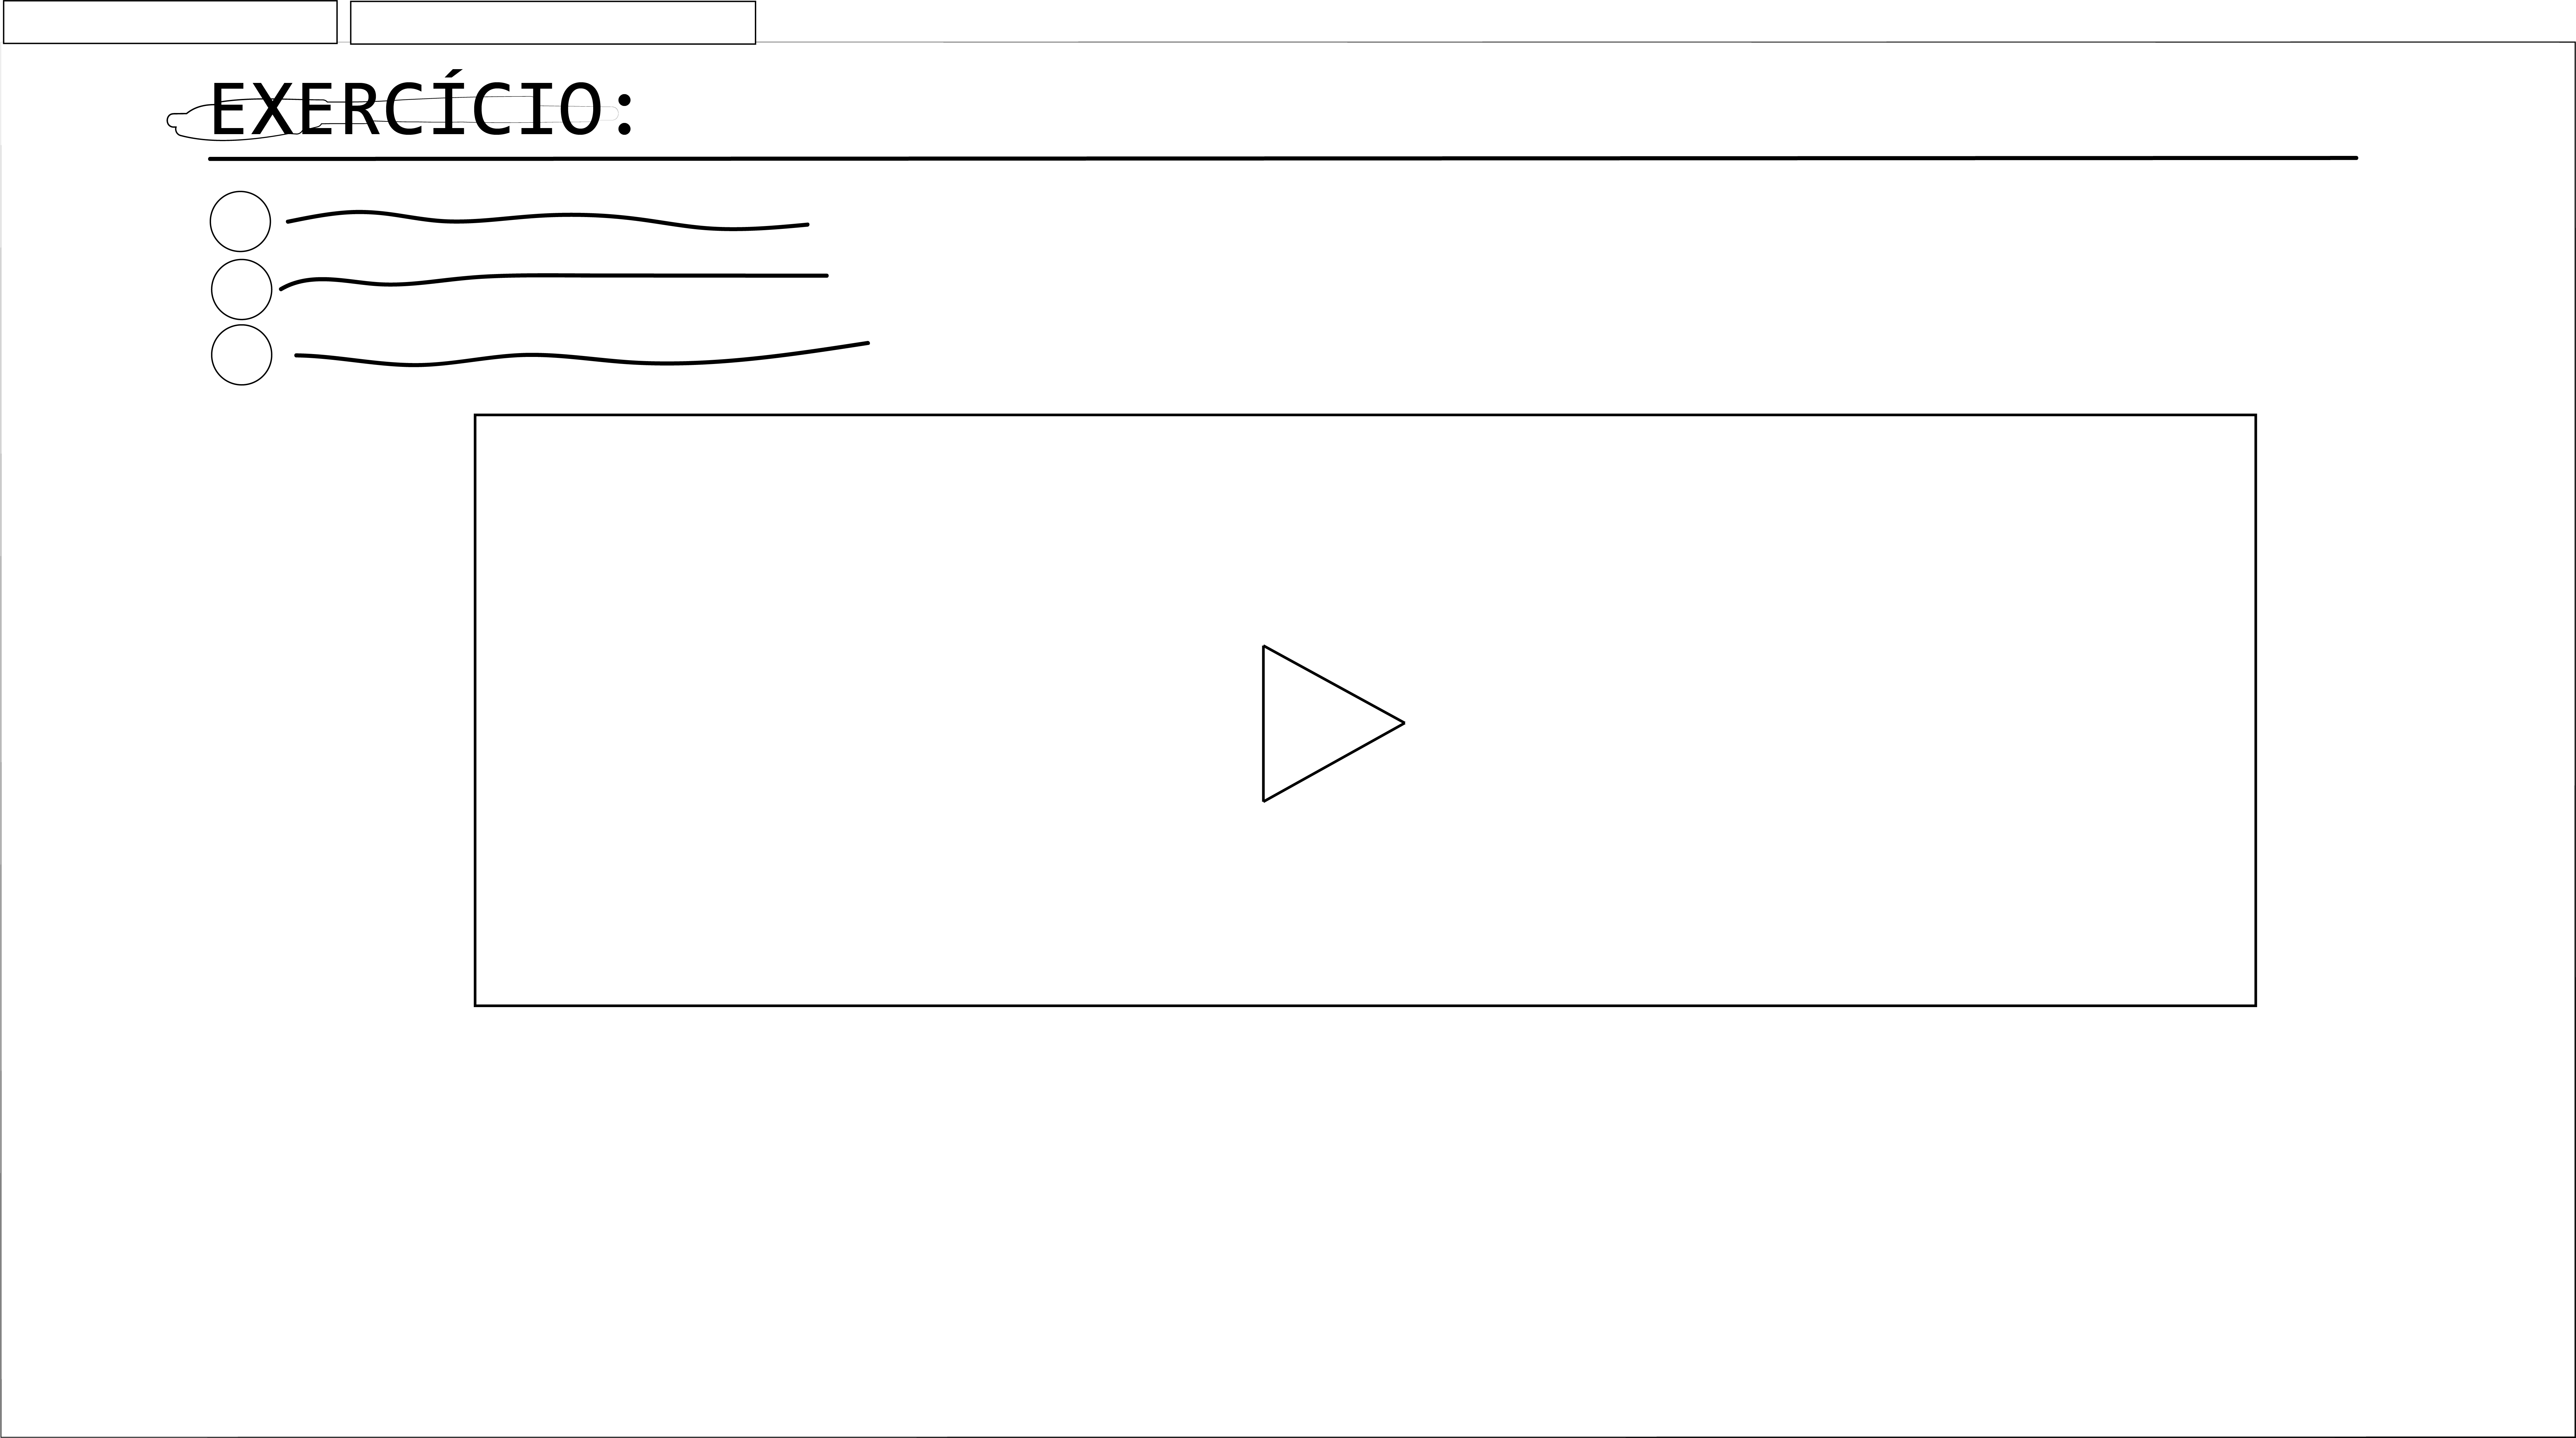
\includegraphics[width=1\textwidth]{img/A.jpg}
    \caption{Esboço da tela de exercícios}
\end{figure}

Podemos ver um projeto de uma barra de navegação para manter os links para outras páginas de forma mais acessível, assim como incluir outras opções importantes, como a opção do modo escuro.

\section{Modo interativo}
Por fim, teremos a última página que poderá ser acessada por um link disponível na barra de navegação e contém a seção de fazer os exercícios informados pelo usuário. O esboço consiste em basicamente um "input" de texto onde será informada uma equação e abaixo será mostrada a resposta ao clicar em um botão. Também é mostrado o gráfico da equação que for informada para melhor visualização e entendimento.

\begin{figure}[H]
    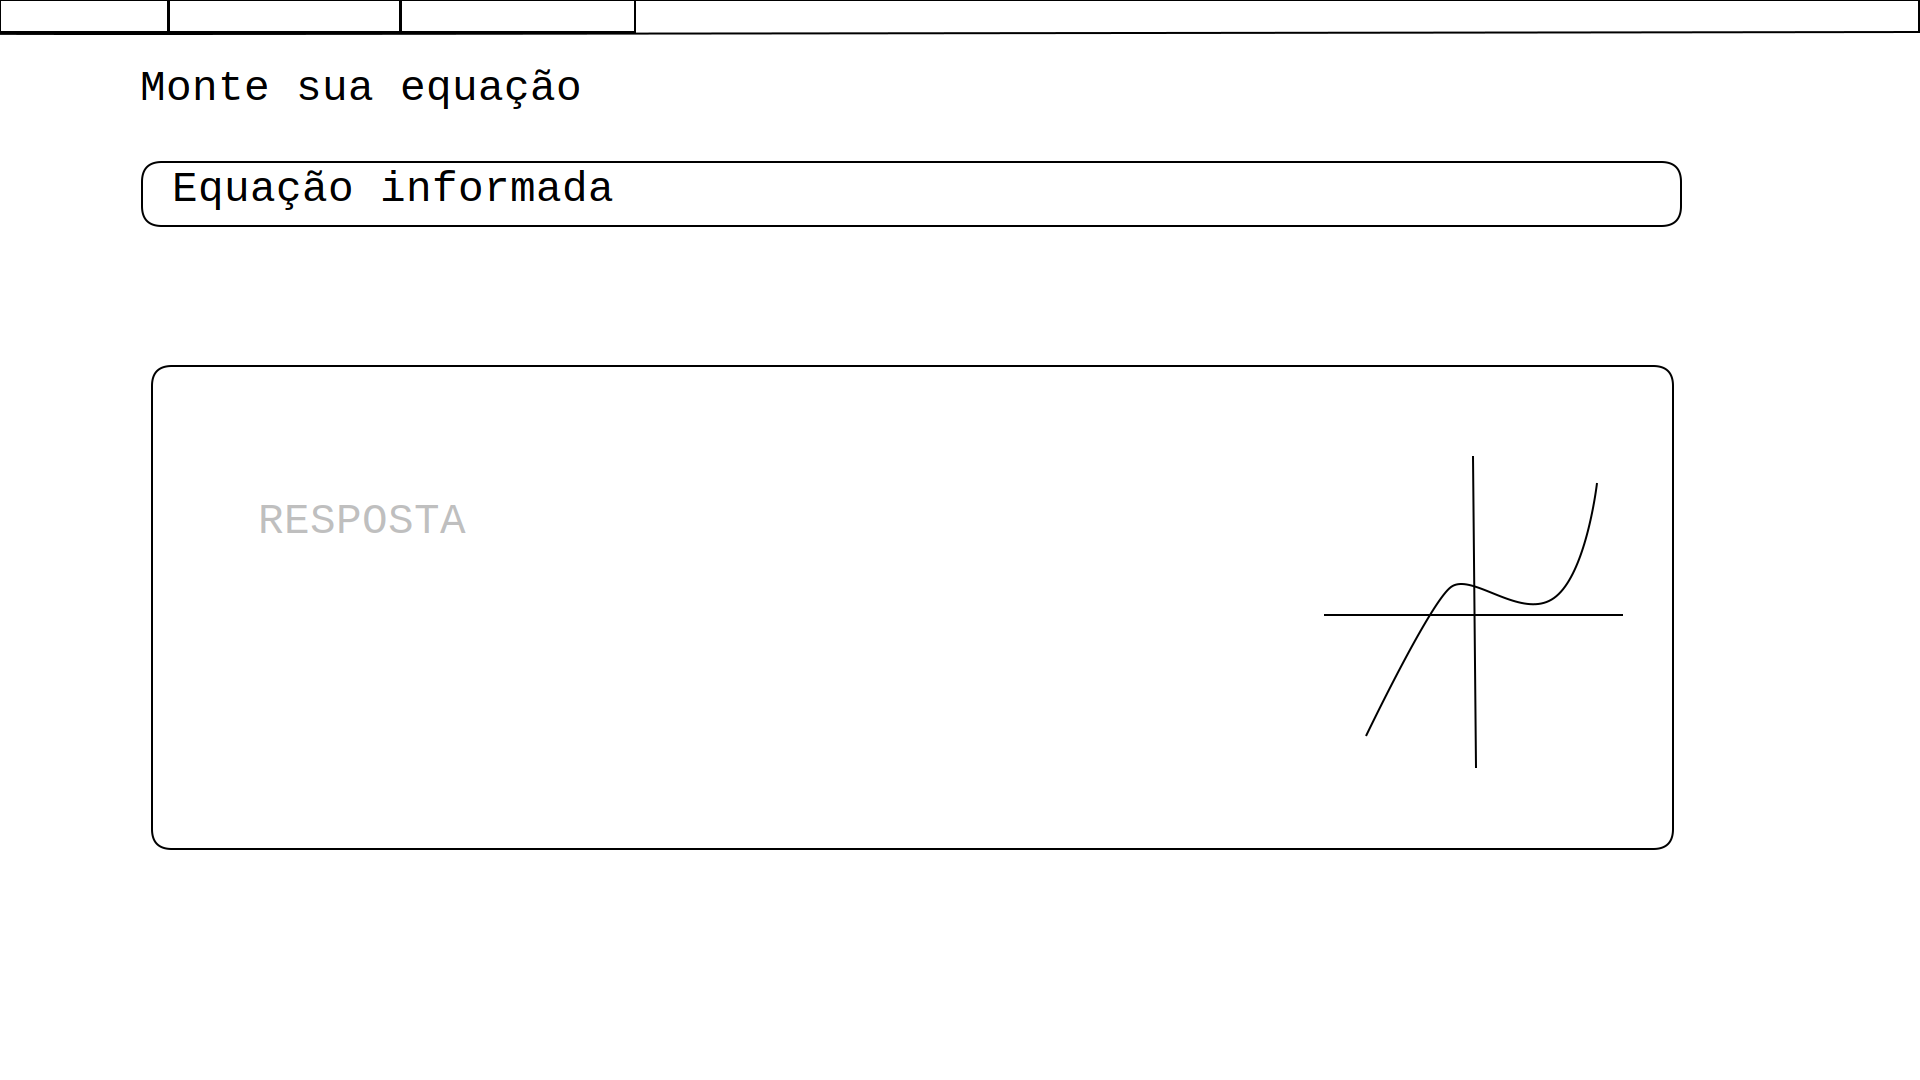
\includegraphics[width=1\textwidth]{img/d.png}
    \caption{Esboço da tela tela de exercícios}
\end{figure}

O portal foi finalizado o desenvolvimento e foram adicionados novos recursos, assim como foi separada a página de conteúdo e exercícios. O esboço mostrado foi o básico do layout que o projeto seguiu.

\chapter{Versão Final}
O portal pode ser acessado pelo link \url{https://pedenite.github.io/PILC-eq/}, onde será acessada a página inicial em sua versão final. O projeto foi desenvolvido com o objetivo de ser open-source e todo o código-fonte do projeto pode ser encontrado em \url{https://github.com/Pedenite/PILC-eq}, incluindo a licença do MIT, que determina as regras de uso e garantia como open-source.

\section{Página inicial}
A \textit{home} do portal possui logo ao início, um vídeo introdutório desenvolvido pelo grupo e, logo em seguida, três botões que servem como links para as outras páginas do portal. Após isso, é possível ver uma introdução às equações em formato de texto, assim como informações sobre o projeto, detalhando o desenvolvimento durante a disciplina e disponibilizando o contato dos autores.

\begin{figure}[H]
    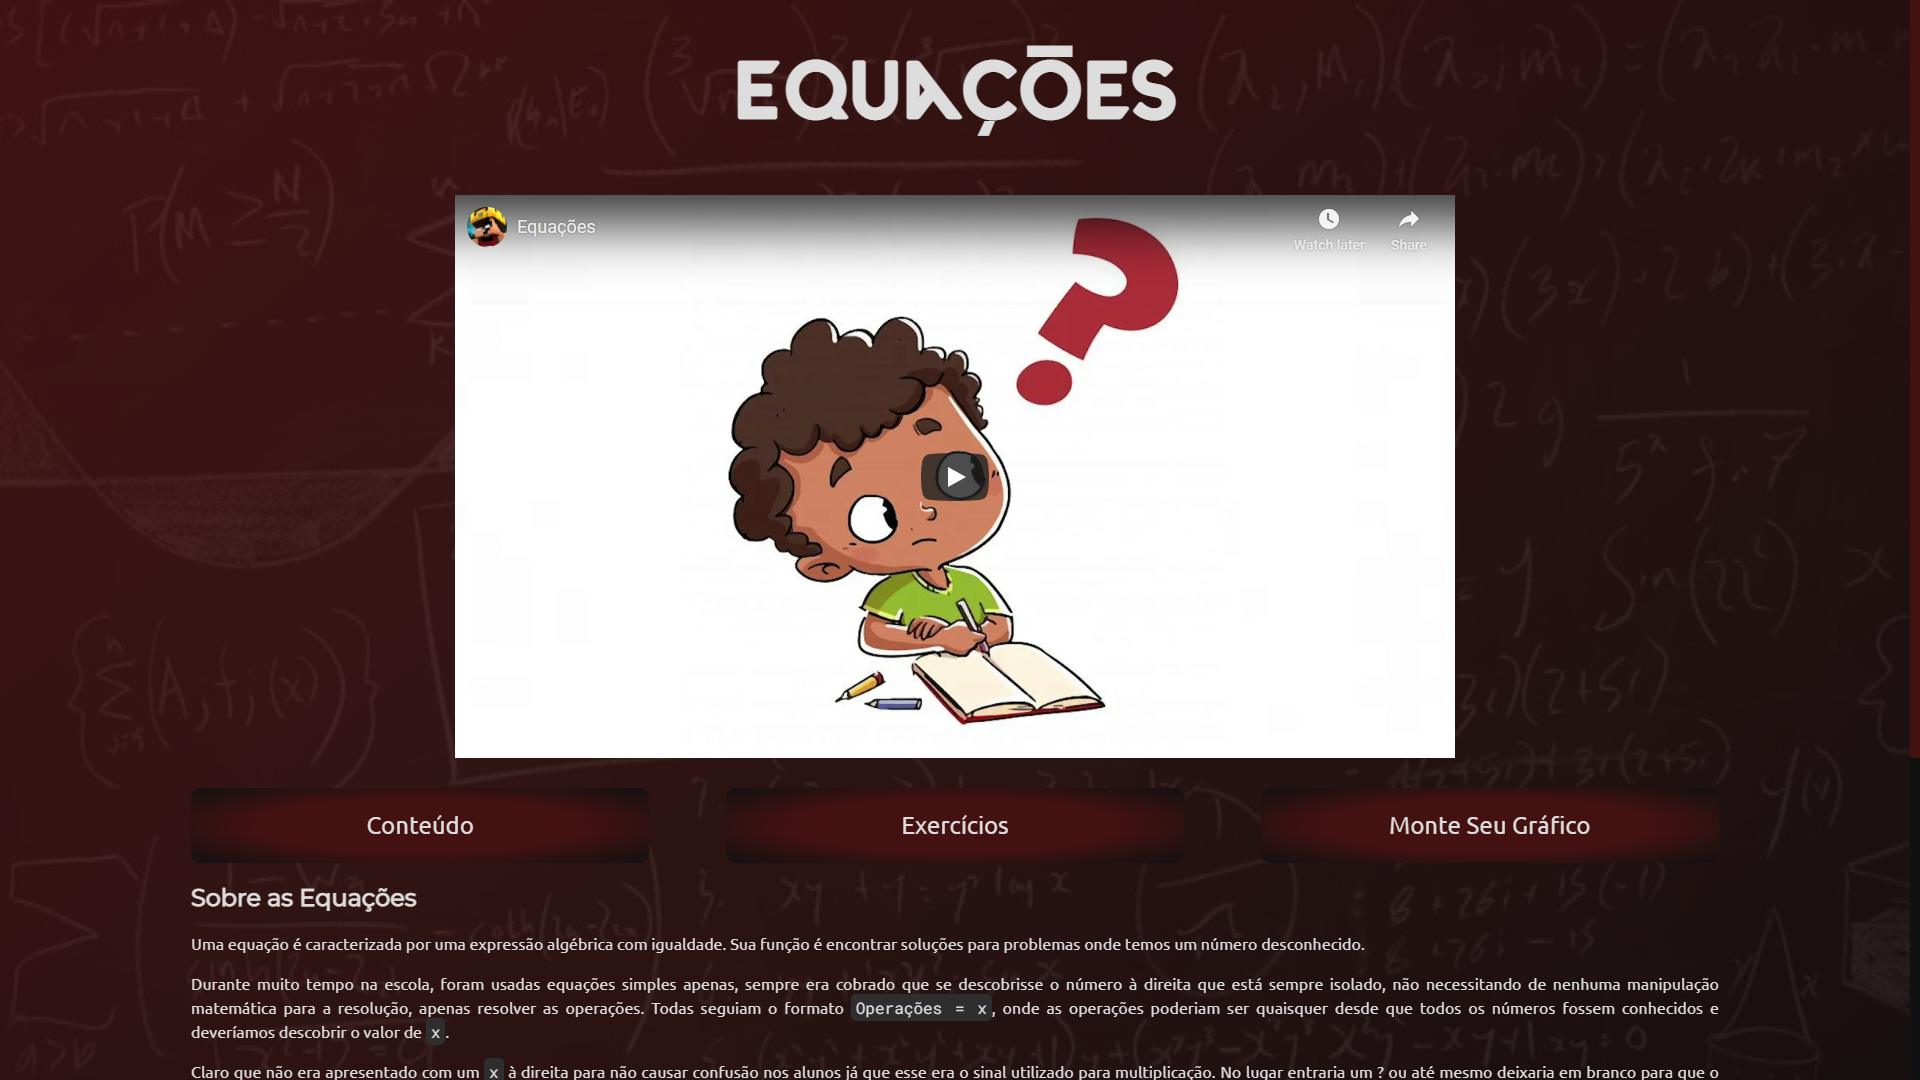
\includegraphics[width=1\textwidth]{img/aplicacao/inicial.png}
    \caption{Página inicial do portal}
\end{figure}

Ao final de todas as páginas é possível encontrar um rodapé simples mostrando a indentificação da disciplina da UnB. Também é disponibilizado o link para o github, onde todos os recursos do site se encontram.

\begin{figure}[H]
    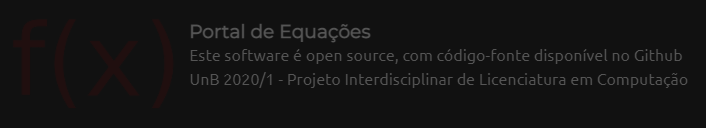
\includegraphics[width=1\textwidth]{img/aplicacao/footer.png}
    \caption{Rodapé do portal}
\end{figure}

\section{Conteúdo}
A segunda página do portal é a página de conteúdo que contém explicações da matéria com pouca quantidade de textos devido à idade o público-alvo, que são adolescentes. Portanto, foram disponibilizadas explicações de outras formas, como imagens, vídeos, gifs e animações.

\begin{figure}[H]
    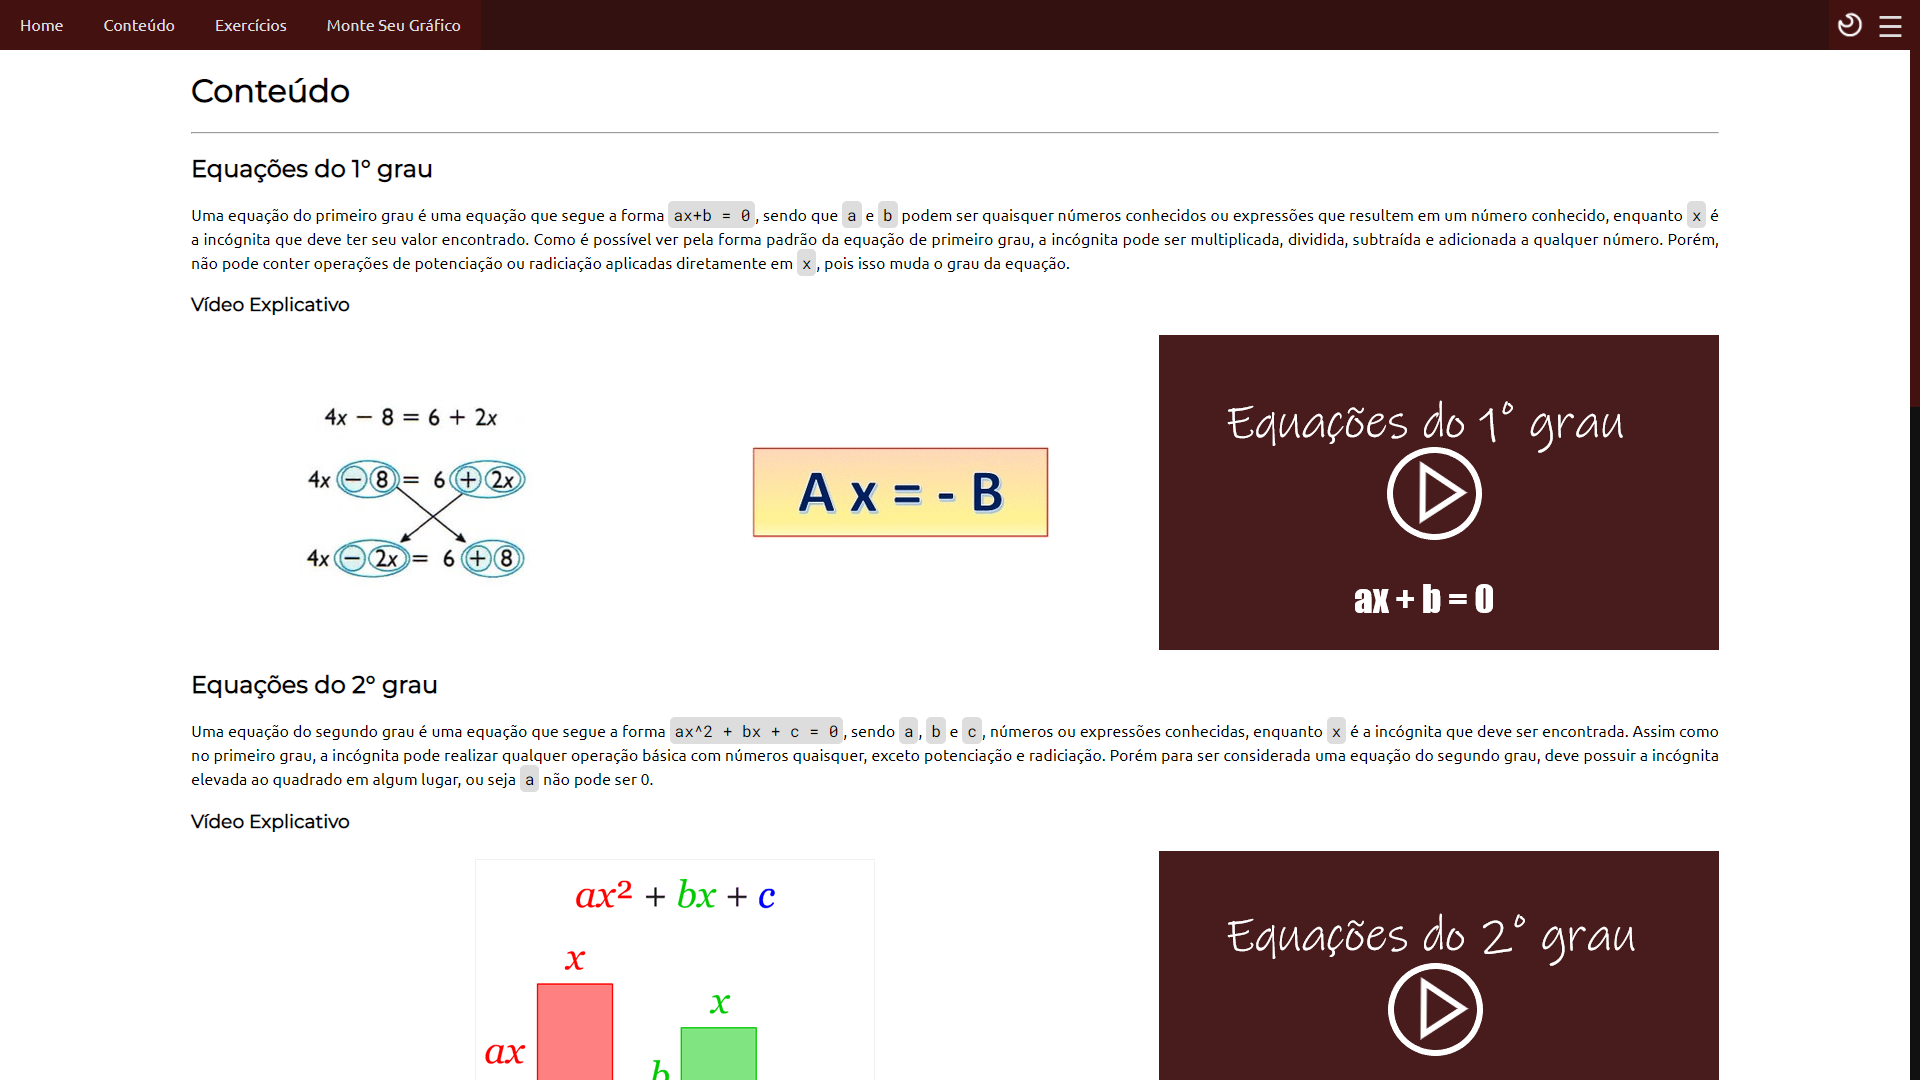
\includegraphics[width=1\textwidth]{img/aplicacao/conteudo_top.png}
    \caption{Página de conteúdo}
\end{figure}

Podemos ver na imagem acima que temos bastante conteúdo sobre as equações de primeiro e segundo grau, incluindo animações para deixar mais intuitivo os materiais apresentados. Porém mais abaixo temos outros conteúdos também, não se limitando somente a isso.

\begin{figure}[H]
    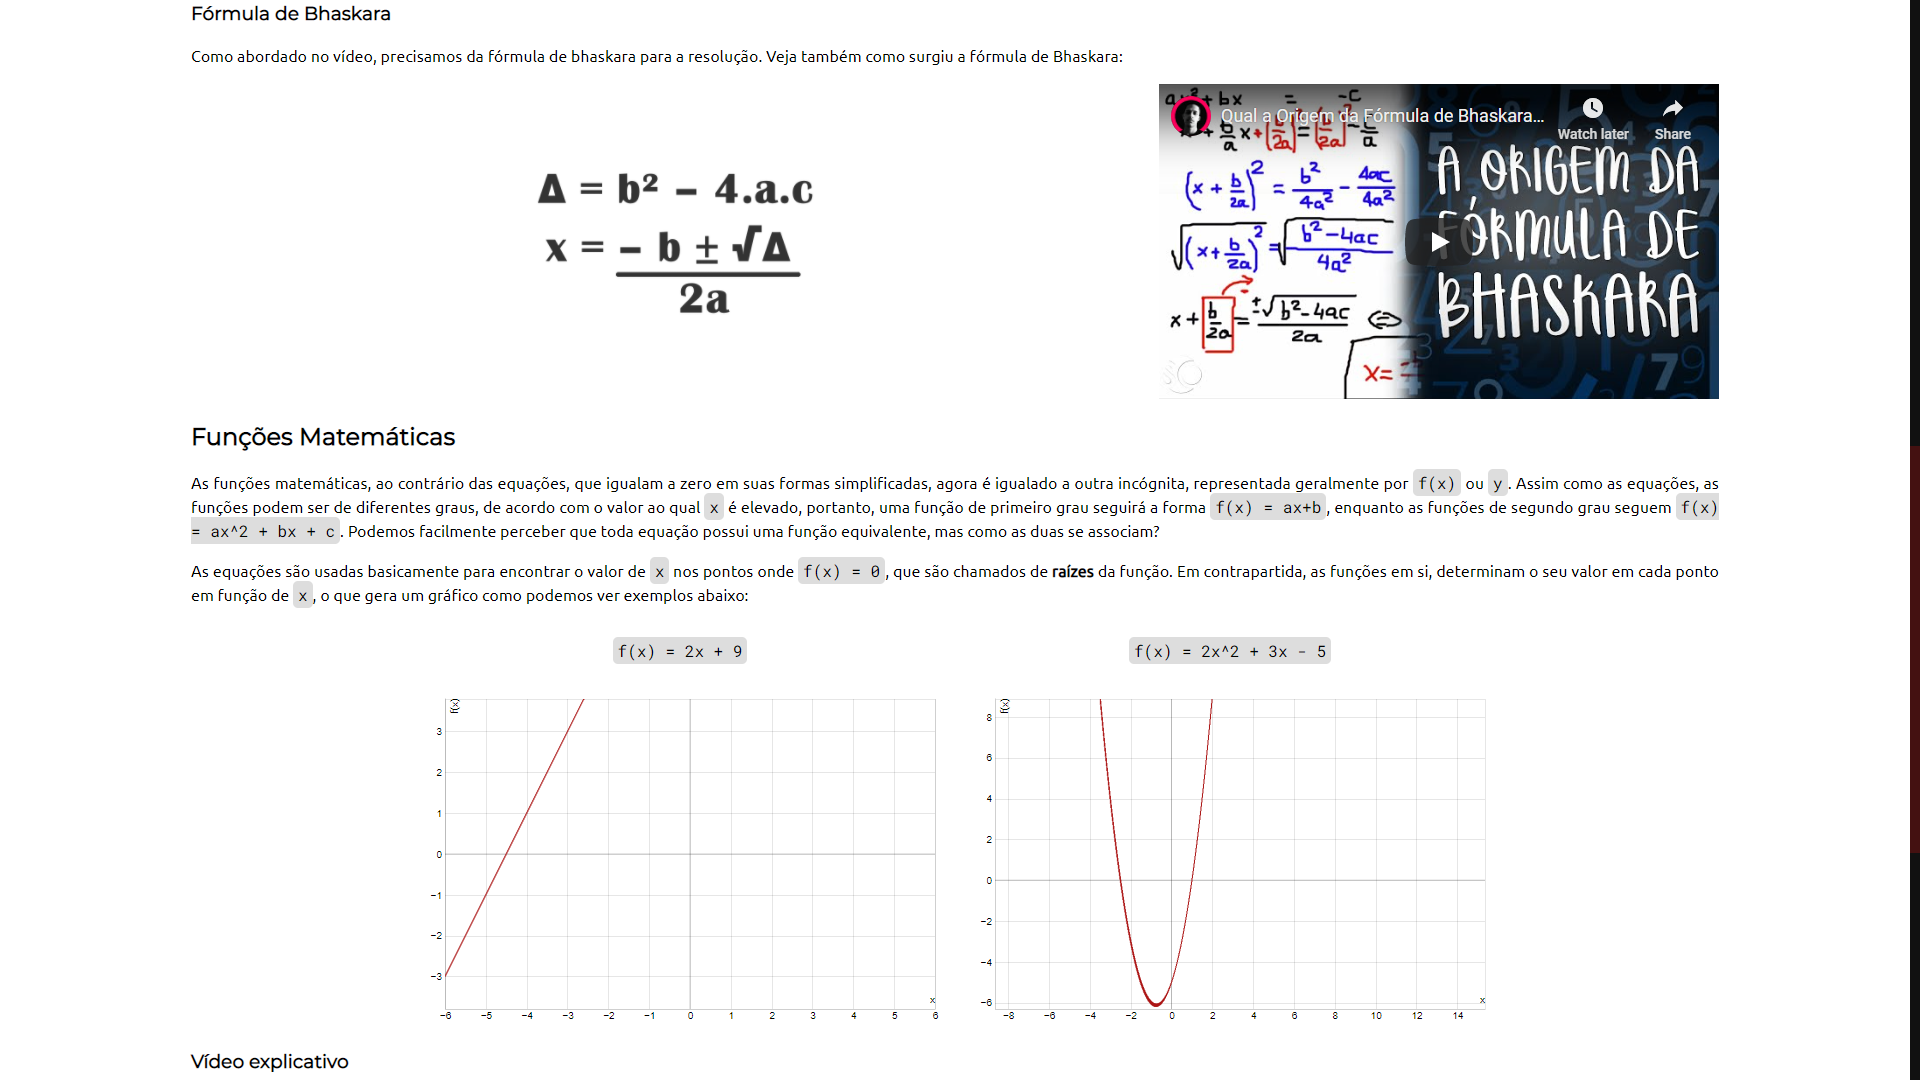
\includegraphics[width=1\textwidth]{img/aplicacao/conteuro_bottom.png}
    \caption{Página de conteúdo mais abaixo}
    \label{conteudo-bottom}
\end{figure}

Vemos que o portal não se limita apenas ao conteúdo de equações, se aproveitando da interdiciplinaridade com outros conteúdos, que está muito presente em diversas áreas. Como mostrado na figura \ref{conteudo-bottom}, podemos ver curiosidades e até gráficos de funções para exemplificar melhor a interpretação e o motivo de se aprender as equações, assim como suas utilidades.

\section{Exercícios}
Na página de exercícios é onde será possível achar uma seleção de problemas matemáticos de equações para que os estudantes possam resolver se assim desejarem. Existem cinco exercícios do primeiro grau e dois do segundo.

\begin{figure}[H]
    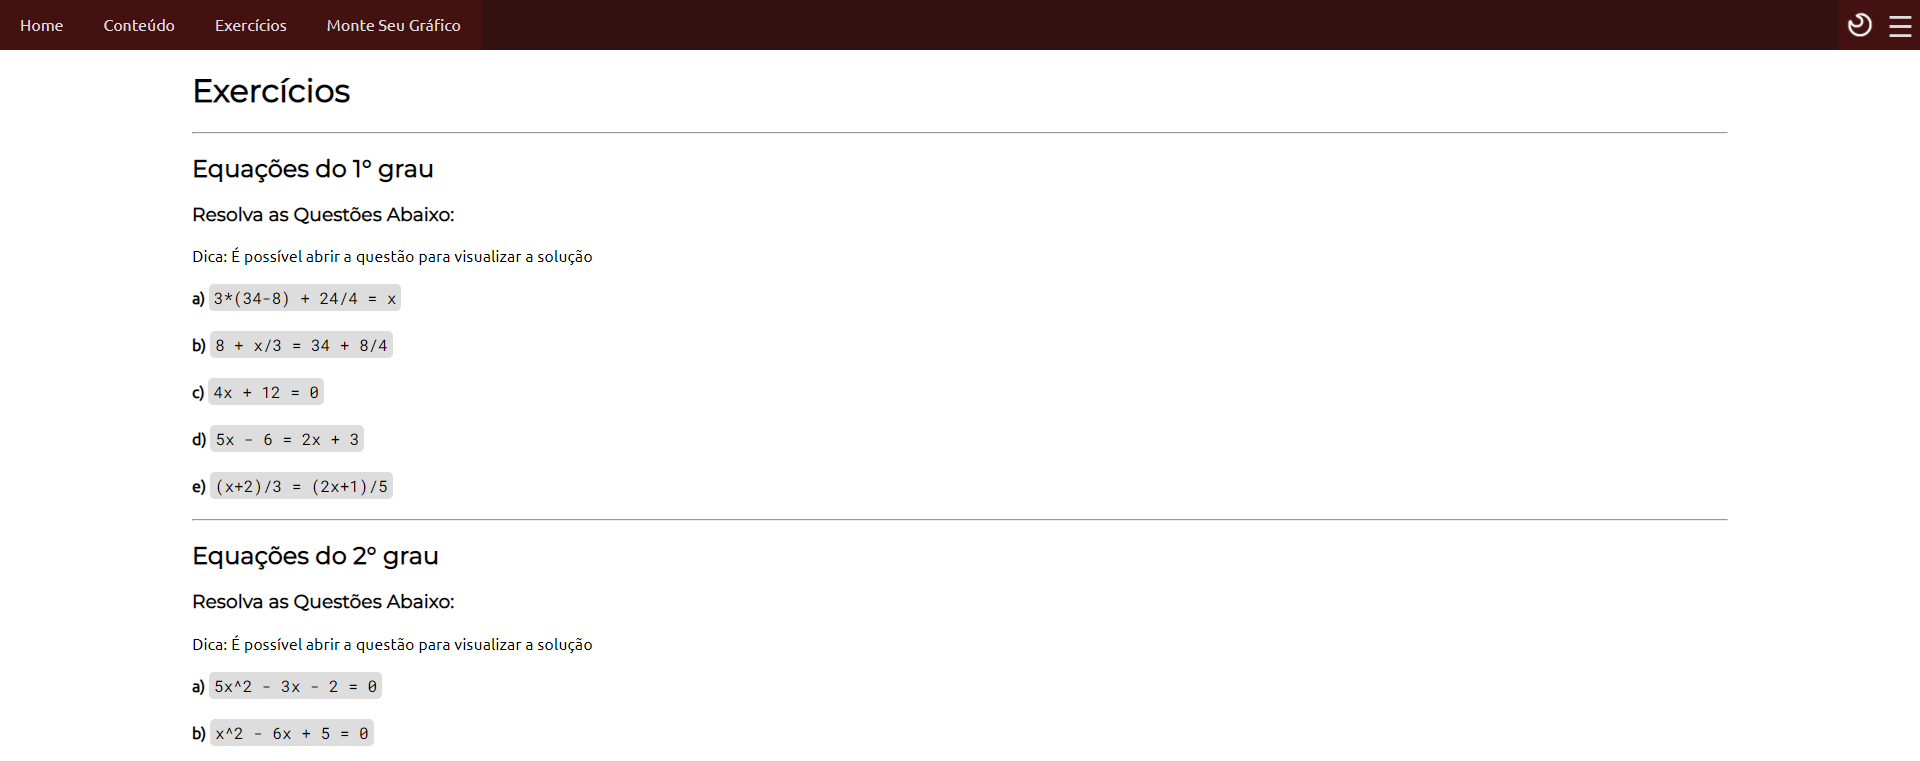
\includegraphics[width=1\textwidth]{img/aplicacao/exercicios.png}
    % \caption{Seleção de exercícios predefinidos}
\end{figure}

Todos os exercícios possuem a opção de serem \textit{clicados} para que seja exibida a solução detalhada passo a passo para que seja conferida a resposta. Para que o aluno fique ciente dessa funcionalidade, existem dicas antes dos exercícios para passar a informação.

\begin{figure}[H]
    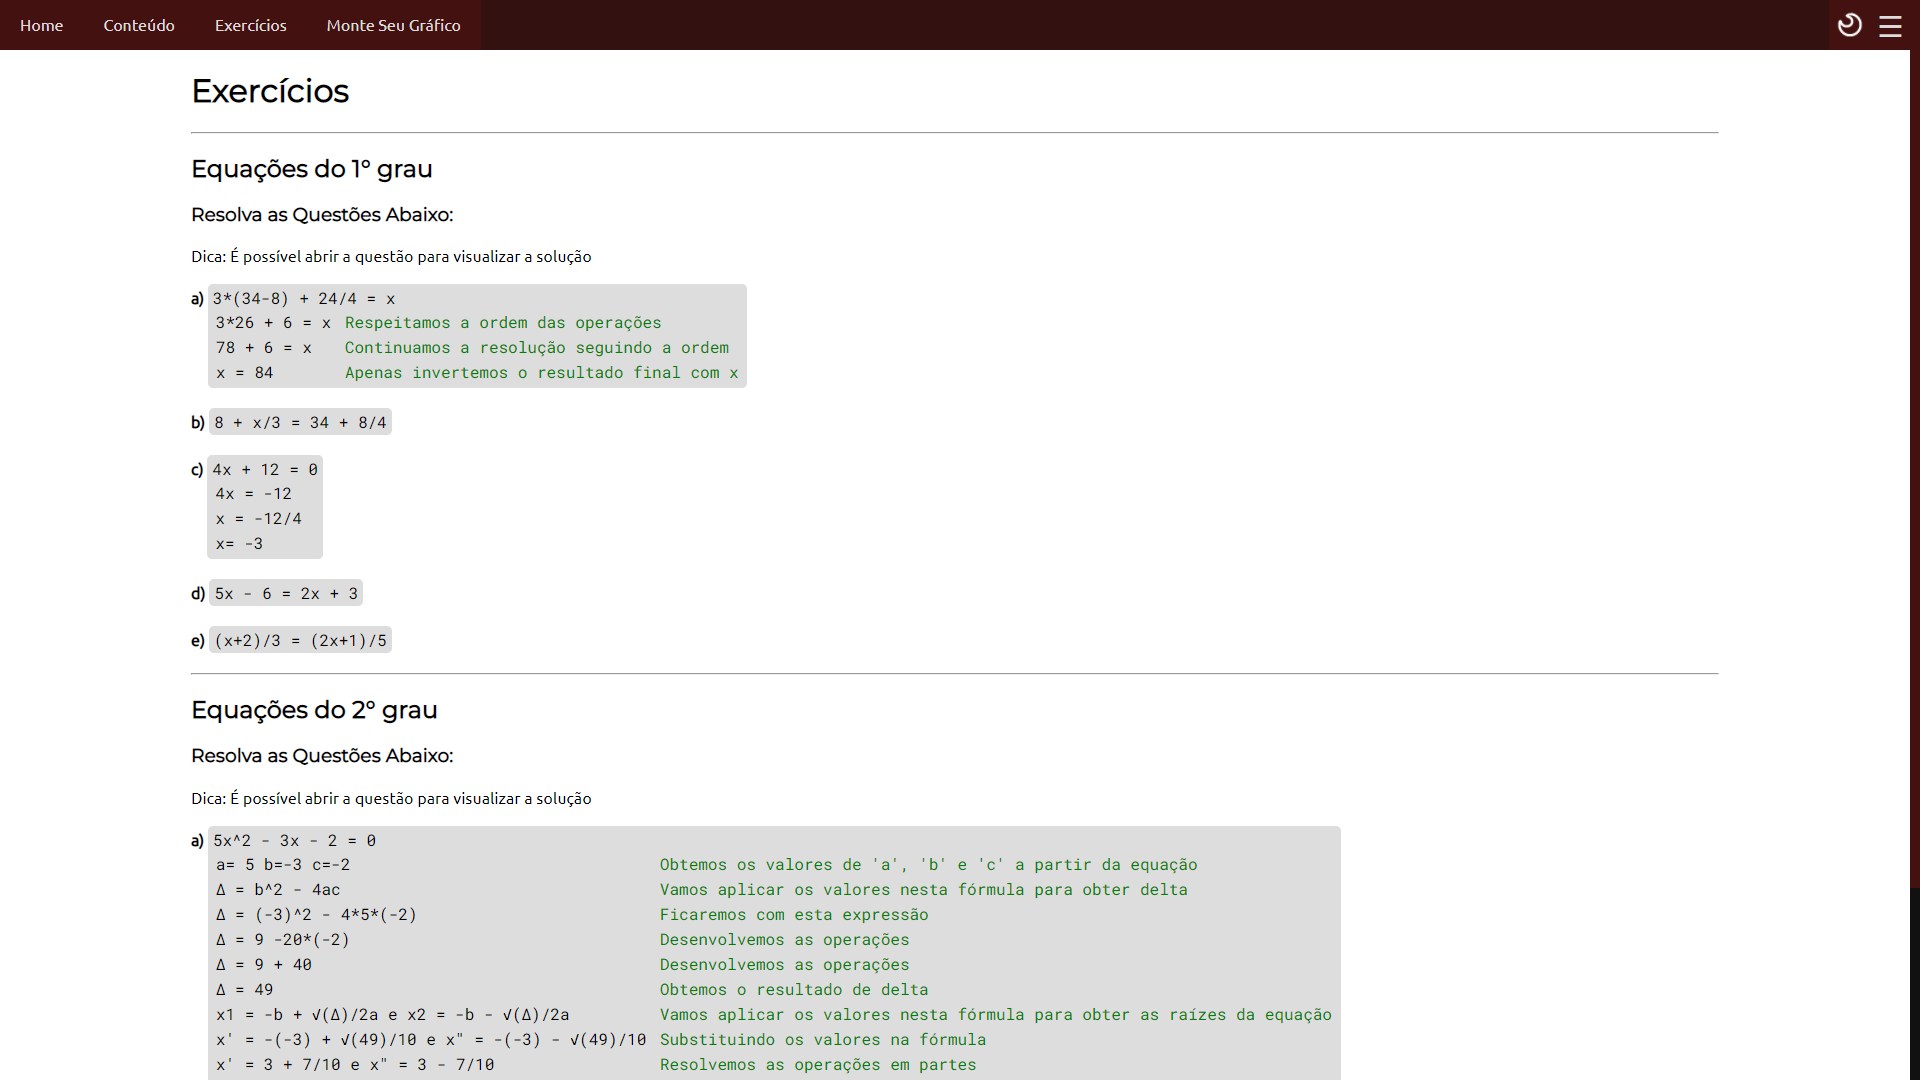
\includegraphics[width=1\textwidth]{img/aplicacao/exercicios_abertos.png}
    \caption{Exercícios com exemplos de soluções abertas}
\end{figure}

\section{Monte Seu Gráfico}
\lipsum[1]

\chapter{Considerações}
Podemos perceber que cada aluno possui sua maneira de estudar e assimilar os conteúdos passados e com o auxílio das ferramentas tecnológicas cada pessoa pode escolher uma que ajude a entender a matéria mais facilmente. O portal em desenvolvimento procura de certa forma, agradar a todo tipo de público, com um visual moderno e a opção de usar temas escuros, tudo para que o usuário sinta-se mais confortavel com a ferramenta, o que é importantíssimo para uma potencialidade no aprendizado.

A interdisciplinaridade, apesar de ainda não incluída no projeto, é um componente importantíssimo do trabalho, que pode ajudar os alunos a compreenderem melhor o conteúdo ao integrá-lo com o mundo real e com outras disciplinas. Serão apresentados conteúdos da física e química para auxiliar no entendimento das equações e da necessidade de seu uso, também podendo auxiliar nas outras disciplinas.

\begin{thebibliography}{9}

\bibitem{Equação do Primeiro Grau}
\noindent Toda Matéria, 
\textit{Equação do Primeiro Grau}
\url{https://www.todamateria.com.br/equacao-do-primeiro-grau/}

\bibitem{Equação do 2° grau}
\noindent Brasil Escola, 
\textit{Equação do 2º grau}
\url{https://brasilescola.uol.com.br/matematica/equacao-2-grau.htm}

\bibitem{Computador na sociendade do conhecimento}
\noindent histórica. In VALENTE, José Armando (org). 
\textit{O computador na sociedade do conhecimento. Campinas: Nied, 2002 Mudanças.}

\bibitem{Interdisciplinaridade: um avanço na educação}
\noindent Meire Cavalcante,
\textit{Interdisciplinaridade: um avanço na educação, 07 de Março de 2018}
\url{https://novaescola.org.br/conteudo/249/interdisciplinaridade-um-avanco-na-educacao?gclid=Cj0KCQjwvvj5BRDkARIsAGD9vlLfazfTkFERfofB1vN-V7rDxoXGWm8athfWhg9VkX2lQnP6Awbh_EsaAnAFEALw_wcB}

\bibitem{Livro interdisciplinaridade}
\noindent Ivani Catarina Arantes Fazenda, Herminia Prado Godoy (2017).
\textit{Interdisciplinaridade: pensar, pesquisar e intervir}

\bibitem{TCC equação do 1 grau}
\noindent José Suelio Lourenço Leite (2019)
\textit{Equações de 1º Grau: A Importância de Práticas Interligadas ao Cotidiano do Aluno}

\end{thebibliography}

\end{document}
